\chapter{Implementing a Monitor Using the \RRH\ Algorithm}
\label{chap:Implementing The Monitor}

This chapter covers the implementation of a monitor that uses the \RRH\ algorithm.  We describe the classes that the monitor is composed of and illustrate the internal structure using UML diagrams.  We show evidence from practical testing that the time required to evaluate a trace in realtime remains constant regardless of trace length when using the reverse algorithm.  From this evidence we conclude that the \RRH\ enables us to construct a monitor that is capable of realtime monitoring.

\section{Monitor Design}
\label{sec:Design}

Our monitor realises the monitor process in the High Level Architecture Diagram \ref{fig:highLevelArchitectureDiagram}, on page \pageref{fig:highLevelArchitectureDiagram} and described in Section \ref{sec:Monitor} of Chapter \ref{chap:Monitoring System Architecture}.

The standard algorithm was implemented ad-hoc and without great attention to code structure.  After the lessons learned from that implementation, it became clear enough what structure the code should take for a worthwhile design to take shape.  The following UML diagrams document the classes within the monitor and the interaction between them when an event is received.

The monitor process receives events generated by the interceptor module embedded into processes by the Xposed framework.  The entry point for events in the monitor process is the EventReceiver class.

\subsection{EventReceiver Class}
\label{sec:EventReceiverClass}

The EventReceiver class is illustrated in Figure \ref{fig:eventReceiverClassDiagram}.  It is responsible for initiating the evaluation of events and reporting on the result.  The class descends from the Android BroadcastReceiver class because events are communicated to the EventReceiver by the Android intent system.  The EventReceiver class registers with the intent system for the type of intent that the interceptor broadcasts.  When the interceptor sends an intent, Android delivers the intent to the EventReceiver by calling the onReceive method with the intent as a parameter.  The EventReceiver extracts details of the event from the intent and begins evaluation.  The EventReceiver is composed of a list of Monitor classes.  In this case, the only monitor in the list is to monitor for the collusion property at the end of Section \ref{sec:ReverseCollusionFormula}.  When monitoring multiple properties, the list gets populated with a different instance of the monitor class for each property.  The EventReceiver calls the Evaluate method of every monitor, and the outcome gets returned as an EvaluationResult.  The EventReceiver reports the result to the user.

%Event Receiver Class Diagram
\begin{figure}[h]
	\centering
	\begin{tikzpicture}[scale=0.7, every node/.style={transform shape}]
	\umlsimpleclass[alias=BroadcastReceiver]{android.content::BroadcastReceiver (abstract)}
	\umlclass[alias=EventReceiver, x=0, y=-3]{com.androidmonitor::EventReceiver}{}{+onReceive(context: Context, intent: Intent): void}
	\umlsimpleclass[alias=monitors, x=0, y=-6]{java.util::ArrayList$<$Monitor$>$}
	\umlclass[alias=Monitor, x=0, y=-9]{RosuHavelund::Monitor}
		{}
		{
			+Evaluate(traceEvent: TraceEvent): EvaluationResult\\
			+Reset(): void
		}
%	\umlsimpleclass[alias=Register, x=0, y=-13]{RosuHavelund::Register}

	\umlinherit{EventReceiver}{BroadcastReceiver}
	\umlcompo[mult1=1, arg2=-monitors, mult2=1]{EventReceiver}{monitors}
	\umluniassoc[mult2=0..n]{monitors}{Monitor}
%	\umlcompo[mult1=1, arg2=-now, mult2=1, anchor1=-130, anchor2=159]{Monitor}{Register}
%	\umlcompo[mult1=1, arg2=-previous, mult2=1, anchor1=-50, anchor2=21]{Monitor}{Register}

	\umlclass[alias=EvaluationResult, x=9, y=-1]{RosuHavelund::EvaluationResult}
		{}
		{
			+Satisfied():boolean\\
			+Message(): String\\
			+SatisfyingEvents() ArrayList$<$TraceEvent$>$
		}
	\umlsimpleclass[alias=satisfyingEvents, x=9, y=-5]{java.util::ArrayList$<$TraceEvent$>$}
	\umlclass[alias=TraceEvent, x=9, y=-9]{RosuHavelund::TraceEvent}
		{}
		{
			+Time():Date\\
			+Event(): String\\
			+Pid(): Int\\
			+AppName(): String\\
			+Action(): String\\
		}

	\umlcompo[mult1=1, arg2=-satisfyingEvents, mult2=1]{EvaluationResult}{satisfyingEvents}
	\umluniassoc[mult2=0..n]{satisfyingEvents}{TraceEvent}

	\end{tikzpicture}
	\caption{Event Receiver Class Diagram}
	\label{fig:eventReceiverClassDiagram}
\end{figure}

\subsection{Monitor Class}
\label{sec:MonitorClass}

The Monitor class is responsible for evaluating a property over a trace event.  Figure \ref{fig:monitorClassDiagram} illustrates the structure of the Monitor in detail.  The reader can observe that the Monitor class implements the \RRH\ algorithm because it is composed of the two registers, \textit{now} and \textit{previous}.  The Evaluate method performs algorithmic steps 1 and 2, described in section \ref{sec:Evaluation} earlier.  Those two steps evaluate the event over the \textit{now} register then update the \textit{previous} register.  The Monitor class returns a positive EvaluationResult if the event satisfies the formula and meets the dynamic conditions.

%Monitor Class Diagram
\begin{figure}[h]
	\centering
	\begin{tikzpicture}[scale=0.66, every node/.style={transform shape}]

		\umlclass[alias=Monitor, x=0, y=0]{RosuHavelund::Monitor}
		{}
		{
			+Monitor(formula: String, message: String, conditions: DynamicConditions)\\
			+Evaluate(traceEvent: TraceEvent): EvaluationResult\\
			+Reset(): void
		}
		
	\umlclass[alias=DynamicConditions, x=12, y=0]{RosuHavelund::DynamicConditions}
		{}
		{
			\umlvirt{\#Met(satisfyingEvents: ArrayList$<$TraceEvent$>$): ArrayList$<$TraceEvent$>$}
		}

	\umlclass[alias=CollusionConditions, x=12, y=-5]{RosuHavelund::CollusionConditions}
		{}
		{
			+Met(satisfyingEvents: ArrayList$<$TraceEvent$>$): ArrayList$<$TraceEvent$>$\\
		}

	\umlclass[alias=Register, x=0, y=-6]{RosuHavelund::Register}
		{}
		{
			+Register(expressions: ArrayList$<$Expression$>$)\\
			+Evaluate(event: String): boolean\\
			+Satisfied(): boolean\\
			+Update(register: Register): void\\
			+Reset(): void
		}

	\umlsimpleclass[alias=expressions, x=0, y=-11]{java.util::ArrayList$<$Expressions$>$}

	\umlclass[alias=Expression, x=0, y=-16]{RosuHavelund::Expression (abstract)}
		{
			+Expression(formula: String, previous: Expression)\\
			+Formula(): String\\
			+Previous(): Expression\\
			+Satisfied(): boolean\\
		}
		{
			+Evaluate(event: String): boolean\\
			+setSatisfied(satisfied: boolean)\\
			+Reset(): void\\
			+FlattenBreadthFirst(): ArrayList$<$Expression$>$
		}
		
	\umlinherit{CollusionConditions}{DynamicConditions}
	\umlcompo[mult1=1, arg2=-now, mult2=1, anchor1=-130, anchor2=121.5]{Monitor}{Register}
	\umlcompo[mult1=1, arg2=-previous, mult2=1, anchor1=-50, anchor2=58]{Monitor}{Register}
	\umlcompo[mult1=1, arg2=-dynamicConditions, pos2=0.7, mult2=1]{Monitor}{CollusionConditions}
	\umlcompo[mult1=1, arg2=-expressions, mult2=1]{Register}{expressions}
	\umluniassoc[mult2=0..n]{expressions}{Expression}

	\end{tikzpicture}
  \caption{Monitor Class Diagram}
  \label{fig:monitorClassDiagram}
\end{figure}

\subsection{Register Class}
\label{sec:RegisterClass}

Registers are arrays where each element corresponds to a subformula in breadth-first order.  The first element corresponds to the root formula, and successive elements correspond to the operands.  An important consideration is that the operands are not always immediately adjacent to the root element in the register.  The following example illustrates this consideration:\\

\begin{myEx} Distant Operands\\

The formula $\varphi = \LTLalwaysbeen((r \,S q) \rightarrow \LTLonce(q \rightarrow \LTLprevious p))$ produces subformulae:

\begin{flushleft}
$ \varphi_{1} = \LTLalwaysbeen((r \,S \,q) \rightarrow \LTLonce(q \rightarrow \LTLprevious p)) $ \\
$ \varphi_{2} = ((r \,S \,q) \rightarrow \LTLonce(q \rightarrow \LTLprevious r)) $ \\
$ \varphi_{3} = (r \,S \,q) $ \\
$ \varphi_{4} = \LTLonce(q \rightarrow \LTLprevious p) $ \\
$ \varphi_{5} = r $ \\
$ \varphi_{6} = q $ \\
$ \varphi_{7} = (q \rightarrow \LTLprevious p) $ \\
$ \varphi_{8} = q $ \\
$ \varphi_{9} = \LTLprevious p $ \\
$ \varphi_{10} = p $ 
\end{flushleft}

The register constructed from those subformulae is:

\begin{tabularx}{\textwidth}{cc|c|c|c|c|c|c|c|c|c|c|}
\centering
 & \multicolumn{1}{c}{}
 & \multicolumn{1}{c}{$ \varphi_{1}$}
 & \multicolumn{1}{c}{$ \varphi_{2}$}
 & \multicolumn{1}{c}{$ \varphi_{3}$}
 & \multicolumn{1}{c}{$ \varphi_{4}$}
 & \multicolumn{1}{c}{$ \varphi_{5}$}
 & \multicolumn{1}{c}{$ \varphi_{6}$}
 & \multicolumn{1}{c}{$ \varphi_{7}$}
 & \multicolumn{1}{c}{$ \varphi_{8}$}
 & \multicolumn{1}{c}{$ \varphi_{9}$}
 & \multicolumn{1}{c}{$ \varphi_{10}$}\\
 \cline{3-12}
 & {now} 
 & { \tikz[baseline]{\node (p1) {$\LTLalwaysbeen$};} } 
 & { \tikz[baseline]{\node (p2) {$\rightarrow$};} }  
 & { \tikz[baseline]{\node (p3) {$ S $};} }
 & { \tikz[baseline]{\node (p4) {$\LTLonce$};} }
 & { \tikz[baseline]{\node (p5) {$r$};} }
 & { \tikz[baseline]{\node (p6) {$q$};} }
 & { \tikz[baseline]{\node (p7) {$\rightarrow$};} }
 & { \tikz[baseline]{\node (p8) {$q$};} }
 & { \tikz[baseline]{\node (p9) {$\LTLprevious$};} }
 & { \tikz[baseline]{\node (p10) {$p$};} } \\
 \cline{3-12}
\end{tabularx}
\begin{tikzpicture}[overlay]
    \draw[red, thick,->] (p1) edge[bend left=10] (p2);
    \draw[red, thick,->] (p2) edge[bend left=10] (p3);
    \draw[red, thick,->] (p2) edge[bend right=30] (p4);
    \draw[red, thick,->] (p3) edge[bend left=30]  (p5);
    \draw[red, thick,->] (p3) edge[bend right=30] (p6);
    \draw[red, thick,->] (p4)[bend left=20] edge (p7);
    \draw[red, thick,->] (p7)[bend left=10] edge (p8);
    \draw[red, thick,->] (p7)[bend right=30] edge (p9);
    \draw[red, thick,->] (p9)[bend left=10] edge (p10);
\end{tikzpicture}
\\\\
The arrows indicate which elements in the register are the operands of another element.  We can see the first element, $\varphi_1$, has the unary has-always-been operator at its root.  In that case, its operand is indeed the adjacent element $\varphi_2$.  But $\varphi_2$ is a binary implies formula with two subformulae as operands.  The satisfaction of $\varphi_2$ is dependent on the immediately adjacent $\varphi_3$ and also on the distant element $\varphi_4$.  And the satisfaction of $\varphi_4$ depends on the satisfaction of distant $\varphi_7$.

\qed
\end{myEx}

To reference the subformulae of a formula is not a trivial exercise of simply referencing the adjacent element in the register.  Instead, the element corresponding to that subformula may be any of the following elements.  When evaluating each element within the register, the challenge is finding the elements corresponding to the operands.  The solution is to make each element of the register a composition that we call an expression.

\subsection{Expression Classes}
\label{sec:ExpressionClasses}

Expressions are responsible for determining the satisfaction of a formula by an event.  They implement operator semantics and present the operands of a formula as references to other expressions.  Every LTL operator we implement has a subclass of expression somewhere within the hierarchical structure shown in class diagram \ref{fig:expressionHierarchy}.

% Expression Hierarchy Class Diagram
\begin{figure}[h!]
	\centering
	\begin{tikzpicture}[scale=0.55, every node/.style={transform shape}]
	
		\umlclass[alias=Expression, x=-8, y=0]{RosuHavelund::Expression (abstract)}
		{
			+Formula(): String\\
			+Previous(): Expression\\
			+Satisfied(): boolean\\
		}
		{
			+Evaluate(event: String): boolean\\
			+setSatisfied(satisfied: boolean)\\
			+Reset(): void\\
			+FlattenBreadthFirst(): ArrayList$<$Expression$>$
		}

		\umlclass[alias=UnaryExpression, x=-2, y=-5]{RosuHavelund::UnaryExpression (abstract)}
		{
			+Operator(): String\\
			+LeftOperand(): Expression\\
		}
		{}
		\umlinherit[geometry=-|]{UnaryExpression}{Expression}

		\umlclass[alias=LiteralExpression, x=-13, y=-5]{RosuHavelund::LiteralExpression}
		{}
		{
			\umlstatic{+Match(formula: String): boolean}\\
			\umlstatic{+MatchPosition(formula: String): int}\\
		}
		\umlinherit[geometry=-|]{LiteralExpression}{Expression}

		\umlclass[alias=BinaryExpression, x=2, y=-9]{RosuHavelund::BinaryExpression (abstract)}
		{
			+RightOperand(): Expression\\
		}
		{}
		\umlinherit[geometry=-|, anchors=180 and -140]{BinaryExpression}{UnaryExpression}

		\umlclass[alias=NotExpression, x=-9, y=-9]{RosuHavelund::NotExpression}
		{}
		{
			\umlstatic{+Match(formula: String): boolean}\\
			\umlstatic{+MatchPosition(formula: String): int}\\
		}
		\umlinherit[geometry=-|, anchors=0 and -140]{NotExpression}{UnaryExpression}

		\umlclass[alias=AlwaysBeenExpression, x=-9, y=-13]{RosuHavelund::AlwaysBeenExpression}
		{}
		{
			\umlstatic{+Match(formula: String): boolean}\\
			\umlstatic{+MatchPosition(formula: String): int}\\
		}
		\umlinherit[geometry=-|, anchors=0 and -140]{AlwaysBeenExpression}{UnaryExpression}

		\umlclass[alias=OnceExpression, x=-9, y=-17]{RosuHavelund::OnceExpression}
		{}
		{
			\umlstatic{+Match(formula: String): boolean}\\
			\umlstatic{+MatchPosition(formula: String): int}\\
		}
		\umlinherit[geometry=-|, anchors=0 and -140]{OnceExpression}{UnaryExpression}

		\umlclass[alias=PreviousExpression, x=-9, y=-21]{RosuHavelund::PreviousExpression}
		{}
		{
			\umlstatic{+Match(formula: String): boolean}\\
			\umlstatic{+MatchPosition(formula: String): int}\\
		}
		\umlinherit[geometry=-|, anchors=0 and -140]{PreviousExpression}{UnaryExpression}
	
		\umlclass[alias=AndExpression, x=6, y=-13]{RosuHavelund::AndExpression}
		{}
		{
			\umlstatic{+Match(formula: String): boolean}\\
			\umlstatic{+MatchPosition(formula: String): int}\\
		}
		\umlinherit[geometry=-|, anchors=180 and -140]{AndExpression}{BinaryExpression}

		\umlclass[alias=OrExpression, x=6, y=-17]{RosuHavelund::OrExpression}
		{}
		{
			\umlstatic{+Match(formula: String): boolean}\\
			\umlstatic{+MatchPosition(formula: String): int}\\
		}
		\umlinherit[geometry=-|, anchors=180 and -140]{OrExpression}{BinaryExpression}

		\umlclass[alias=ImpliesExpression, x=6, y=-21]{RosuHavelund::ImpliesExpression}
		{}
		{
			\umlstatic{+Match(formula: String): boolean}\\
			\umlstatic{+MatchPosition(formula: String): int}\\
		}
		\umlinherit[geometry=-|, anchors=180 and -140]{ImpliesExpression}{BinaryExpression}
		
		\umlclass[alias=SinceExpression, x=6, y=-25]{RosuHavelund::SinceExpression}
		{}
		{
			\umlstatic{+Match(formula: String): boolean}\\
			\umlstatic{+MatchPosition(formula: String): int}\\
		}
		\umlinherit[geometry=-|, anchors=180 and -140]{SinceExpression}{BinaryExpression}
	\end{tikzpicture}
 	\caption{Expression Hierarchy}
 	\label{fig:expressionHierarchy}
\end{figure}

At the top level of the class hierarchy, there is an abstract expression class composed of a formula string, a boolean to indicate if an event satisfies that formula, and a reference to the same expression in the \textit{previous} register.  Temporal operators make use of the Previous expression during evaluation.  Literal expressions and unary expressions are extensions of the abstract expression class.  Literals have no operator or operands, and unary expressions have an operator and a left operand.  Binary expressions are a derivative of unary expressions and add the right operand.  The operands of an expression are references to other expressions within the register and Section \ref{sec:MonitorConstruction} will describe how they get made.  

All expressions have an Evaluate method responsible for returning whether the event parameter satisfies that expressions formula, according to the semantics of the outermost operator.

\subsection{Monitor Construction}
\label{sec:MonitorConstruction}

When the monitor process gets launched, the process entry point constructs a monitor for the collusion formula defined in Section \ref{sec:ReverseCollusionFormula}.  The collusion formula and an instance of the dynamic conditions related to that formula get passed to the monitor's constructor.  Instantiation of the monitor class begins a cascade of object instantiations that result in the structure shown in Figure \ref{fig:monitorClassDiagram}.

The monitor class uses a class factory to construct two syntax trees from the formula.  The class factory contains all the concrete subclasses of the expression class shown in Figure \ref{fig:expressionHierarchy}.  It returns an instance of the expression whose operator is at the root of the formula.  The class factory does this by iterating through the registered expression classes, calling the static match method on each, until it finds the expression whose operator matches the outermost\footnote{The outermost operator gets identified as the operator outside all braces} operator of the formula.  The match method is static because we do not wish to construct an instance of the class only to discover the operator does not match the operator of the formula.  When the matching expression gets found, the class factory constructs an instance and passes the formula string to the constructor.  The expression constructor recognises the formula operands as the substrings to the left and right of the outermost operator.  It constructs child expressions for the operands by calling the class factory again with each substring.  Syntax tree construction recurses until it reaches leaf nodes with no operator or operands.  The class factory then constructs a literal class with no child nodes, and the syntax tree is complete.

Monitor constructor then continues by creating the \textit{now} and \textit{previous} registers from the tree structures.  Each tree gets flattened into a breadth-first ordered array of expressions by calling the flatten method on the root node of each tree.  The flatten method traverses the tree in breadth-first order and puts each node into an array.  As mentioned earlier, the operands of each expression are references to child expressions in the tree.  After the tree gets flattened into an array, the references point to other array elements.  It is then easy to reach operands elsewhere in the register.

The semantics of the temporal operators, such as has-always-been and once, involve earlier evaluations.  The \textit{previous} register keeps track of earlier evaluations therefore the \textit{now} register needs a reference to it.  The syntax tree for the \textit{previous} register gets constructed first, and the root expression gets passed to the constructor of the \textit{now} tree that is constructed second.  As each node in the \textit{now} tree is constructed, the \textit{previous} tree is traversed in unison.  A reference to the corresponding node from the \textit{previous} tree is passed to the constructor of each \textit{now} tree node and held.  The reference is called Previous and can be seen in the expression class in Figures \ref{fig:monitorClassDiagram} and \ref{fig:expressionHierarchy}.  When the trees get flattened into registers, the expressions from the \textit{previous} register are available to the corresponding expressions in the \textit{now} register during evaluation.

\subsection{Performing an Evaluation}
\label{sec:PerformingAnEvaluation}

The sequence diagram in Figure \ref{fig:monitorSequenceDiagram} illustrates the evaluation of an event in detail.  The EventReceiver class in the monitor process receives an event from the interceptor.  The EventReceiver passes the event to the monitor by calling its Evaluate method.  In turn, the monitor delegates evaluation to its \textit{now} register by calling its Evaluate method.  The \textit{now} register iterates through each expression, from the last to the first, calling the expression's Evaluate method and passing the event.  The result of the expression's Evaluate method gets determined by the semantics of the expression's operator from Definition \ref{def:PastNon-emptyTraceSemantics}.  The result gets assigned to the expression's Satisfied member and returned to the register.

After the event has been evaluated by all expressions within the \textit{now} register, execution returns to the monitor.  The result of evaluating over the \textit{now} register gets accumulated into the \textit{previous} register by calling the Update method on the \textit{previous} register and passing the \textit{now} register.  The Update method iterates through all the expressions within the \textit{previous} register and assigns a value to the Satisfied member from the corresponding member in the \textit{next} register.

After updating the \textit{previous} register, the Evaluate method of the monitor is complete, and it returns an EvaluationResult to the EventReceiver.  The EvaluationResult comprises a boolean to indicate satisfaction of the formula and the list of events that contributed to satisfaction.

If the EvaluationResult confirms the formula is satisfied, the user gets notified that possible collusion is detected.  The monitor then gets reset so that it can recognise more collusion attacks.  It gets reset by assigning values to the Satisfied members of expressions in the \textit{now} and \textit{previous} registers that are arrived at when evaluating an empty trace.  The effect is that the monitor will continue as if it has never seen any events.  It will recognise future attacks but not recognise attacks in progress when the monitor got satisfied.  An alternative method to reset the monitor is to remove the events that satisfied the monitor from the trace, and reevaluate the remaining trace.  The monitor would then recognise other collusion attacks in progress when the monitor was satisfied as well as future attacks.

% Event evaluation sequence diagram
\begin{figure}[h]
	\begin{resizedtikzpicture}{\textwidth}
		\begin{umlseqdiag}
		\umlactor[class=Process]{app}
		\umlobject[class=Interceptor]{interceptor}
		\umlactor[class=Process]{monitorProcess}
		\umlobject[class=EventReceiver]{receiver}
		\umlmulti[class=Monitor]{monitor}
		\umlmulti[class=Register]{register}
		\umlmulti[class=Expression]{expression}
		\umlobject[class=CollusionConditions, x=30]{dynamicConditions}
		\begin{umlcall}[op={action}]{app}{interceptor}
			\begin{umlcall}[op={intent}]{interceptor}{monitorProcess}
				\begin{umlcall}[op={onReceive(intent)}]{monitorProcess}{receiver}
		
					\begin{umlfragment}[type=loop, label=foreach monitor]
					
						\begin{umlcall}[op={Evaluate(event)}, return=result]{receiver}{monitor}
							\begin{umlcall}[op={now.Evaluate(event)}, return=result]{monitor}{register}
								\begin{umlfragment}[type=loop, label=foreach expression, inner xsep=7]
									\begin{umlcall}[op={Evaluate(event)}, return=result]{register}{expression}\end{umlcall}
								\end{umlfragment}
							\end{umlcall}
							\begin{umlcall}[op={previous.Update()}]{monitor}{register}\end{umlcall}
							
							\begin{umlfragment}[type=opt, label=if previous.Satisfied, inner xsep=7]
								\begin{umlcall}[op={Met(satisfyingEvents)}, return=satisfyingEvents]{monitor}{dynamicConditions}\end{umlcall}			
							\end{umlfragment}
						\end{umlcall}
					
						\begin{umlfragment}[type=opt, label=if result.Satisfied, inner xsep=4]
							\begin{umlcall}[op={Reset()}]{receiver}{monitor}
								\begin{umlcall}[op={now.Reset()}]{monitor}{register}
									\begin{umlfragment}[type=loop, label=foreach expression, inner xsep=7]
										\begin{umlcall}[op={Reset()}]{register}{expression}\end{umlcall}
									\end{umlfragment}
								\end{umlcall}
								
								\begin{umlcall}[op={previous.Reset()}]{monitor}{register}
									\begin{umlfragment}[type=loop, label=foreach expression, inner xsep=7]
										\begin{umlcall}[op={Reset()}]{register}{expression}\end{umlcall}
									\end{umlfragment}
								\end{umlcall}
							\end{umlcall}
						\end{umlfragment}
						
					\end{umlfragment}
			\end{umlcall}
			\end{umlcall}
		\end{umlcall}
		\end{umlseqdiag}
	\end{resizedtikzpicture}
    \caption{Evaluation of an Action}
    \label{fig:monitorSequenceDiagram}
\end{figure}

\section{Testing the \RRH\ Algorithm}
\label{sec:Testing The Reverse Rosu-Havelund Algorithm}

We performed similar functional tests on the reverse algorithm to those for the standard \RH\ algorithm, except that tests for future operators got replaced with tests for past operators.

Test cases got generated manually by applying the semantics of each operator, from section \ref{sec:LTLPastSemantics} to a series of traces and noting the expected result.  The test cases are in appendix \ref{app:RRHFunctionalTestCases}.  For practical use, it was necessary to replace some of the LTL symbols with characters available on the keyboard.  Table \ref{tab:AlternativeLTLOperators} provides the translation.

The tests were run by entering the formula and test traces from each test case into a test harness application.  The test harness then evaluated the formula over each trace using the \RRH\ implementation and wrote the results to the console window.  The results are in appendix \ref{app:RRHFunctionalTestResults} and the test harness code is in \ref{app:RRHCode}.  The results confirm the functionality is identical to that of the standard algorithm with respect to the classical logical operators and the functioning of the past temporal operators is as expected.

We also ran the same performance tests as those in section \ref{subsec:PracticalPerformanceAnalysisExecution} on the \RRH\ algorithm.  We used the reader and publisher apps to generate traces of increasing length and measured the time taken to evaluate each trace.

\subsection{Test Results}
\label{subsec:PracticalPerformanceAnalysisResultsRRH}

Table \ref{tab:ReverseRHExecutionTimes} gives the performance test results.  The time taken to evaluate each trace remained constant at less than a second, regardless of the size of the trace.

\begin{table}[h!]
	\centering
	\captionsetup{width=0.6\linewidth, justification=centering}
	\begin{tabular}{r|r} 
	Trace Length  & Duration\\
	(collusion sequences) & (seconds)\\
	\hline
	10 & $<1$\\
	20 & $<1$\\
	30 & $<1$\\
	40 & $<1$\\
	50 & $<1$\\
	60 & $<1$\\
	70 & $<1$\\
	80 & $<1$\\
	90 & $<1$\\
	100 & $<1$\\
	\hline
	\end{tabular}
	\caption{Duration of the \RRH\ Algorithm Evaluating Traces of Increasing Length}
	\label{tab:ReverseRHExecutionTimes}
\end{table}

%\newpage

\section{Scalability of the \RRH\ Algorithm}
\label{sec:Scalability Of Reverse Rosu-Havelund Algorithm}

Figure \ref{fig:ReverseRHEvaluationDuration} compares the performance of the standard \RH\ algorithm, plotted by the blue curve, with that of the \RRH\ algorithm, plotted by the flat green curve.  The results are in line with our expectations of the reverse algorithm and support its suitability for realtime monitoring.

\begin{figure}[h!]
	\centering
	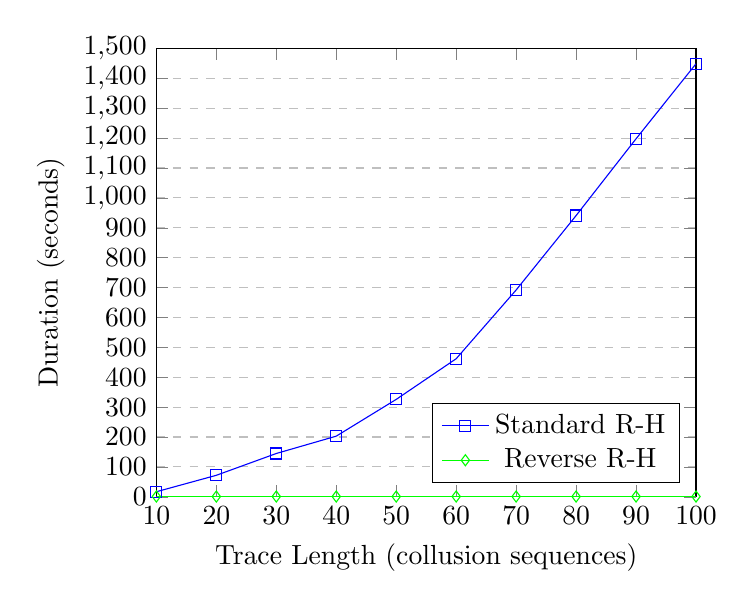
\begin{tikzpicture}
	\begin{axis}[
	    xlabel={Trace Length (collusion sequences)},
	    ylabel={Duration (seconds)},
	    xmin=10, xmax=100,
	    ymin=0, ymax=1500,
	    xtick={10,20,30,40,50,60,70,80,90,100},
	    ytick={0,100,200,300,400,500,600,700,800,900,1000,1100,1200,1300,1400,1500},
	    legend pos=south east,
	    ymajorgrids=true,
	    grid style=dashed,
	]
	
	\addplot[
	    color=blue,
	    mark=square,
	    ]
	    coordinates {
	    (10,17)(20,72)(30,145)(40,203)(50,326)(60,462)(70,692)(80,941)(90,1198)(100,1449)
	    };
	    \addlegendentry{Standard R-H}
	    
	\addplot[
	    color=green,
	    mark=diamond,
	    ]
	    coordinates {
	    (10,1)(20,1)(30,1)(40,1)(50,1)(60,1)(70,1)(80,1)(90,1)(100,1)
	    };
		\addlegendentry{Reverse R-H}
	\end{axis}
	\end{tikzpicture}
	\caption{Dependency Between Trace Length and Evaluation Duration}
	\label{fig:ReverseRHEvaluationDuration}
\end{figure}